\section{Problem 2: GAN Synthetic Data with Low-Data Stabilization}

\subsection{Objective}
Similar to Problem 1, this section evaluates a Conditional Generative Adversarial Network (cDCGAN) trained on 350 real examples per digit. The goal is to determine if GAN-generated synthetic samples can effectively stabilize a model trained in a low-data regime, and to find the best confidence selection strategy.

\subsection{Methodology}
\begin{enumerate}
    \item \textbf{Augmentation:} The initial 350 real examples were augmented.
    \item \textbf{Training the GAN:} A cDCGAN was trained on the augmented dataset.
    \item \textbf{Generation:} 50,000 synthetic samples were generated.
    \item \textbf{Confidence Filtering:} The generated samples were passed through the LeNet-5 classifier to categorize them into Set A (All), Set B (High Confidence), and Set C (Mid Confidence).
\end{enumerate}

\subsection{Results \& Conclusion}
The results for the GAN generations are documented in Table \ref{tab:vae_gan_comparison} under the VAE section. 

\textit{Question: Which GAN selection strategy gives the best improvement, and does GAN-generated data reduce the need for real data?}

\textbf{Answer:} 
\begin{itemize}
    \item \textbf{Best Selection Strategy:} \textbf{Set C (Mid Confidence, 0.6 $\leq$ CL $\leq$ 0.9)} provided the best accuracy improvement (93.45\%). Similar to the VAE, these samples act as effective regularizers. They are slightly ambiguous but semantically correct, pushing the LeNet-5 classifier to refine its decision boundaries.
    \item \textbf{Reducing the need for real data:} \textbf{Partially, but not completely.} While GAN-generated data improved the baseline 350-real performance (jumping up to 93.45\%), it could \textbf{not} beat the pure 1000-Real data baseline, which achieved 97.50\% test accuracy. Therefore, while synthetic data helps in a strict low-data regime, genuine real-world data remains vastly superior.
\end{itemize}

\begin{figure}[h!]
    \centering
    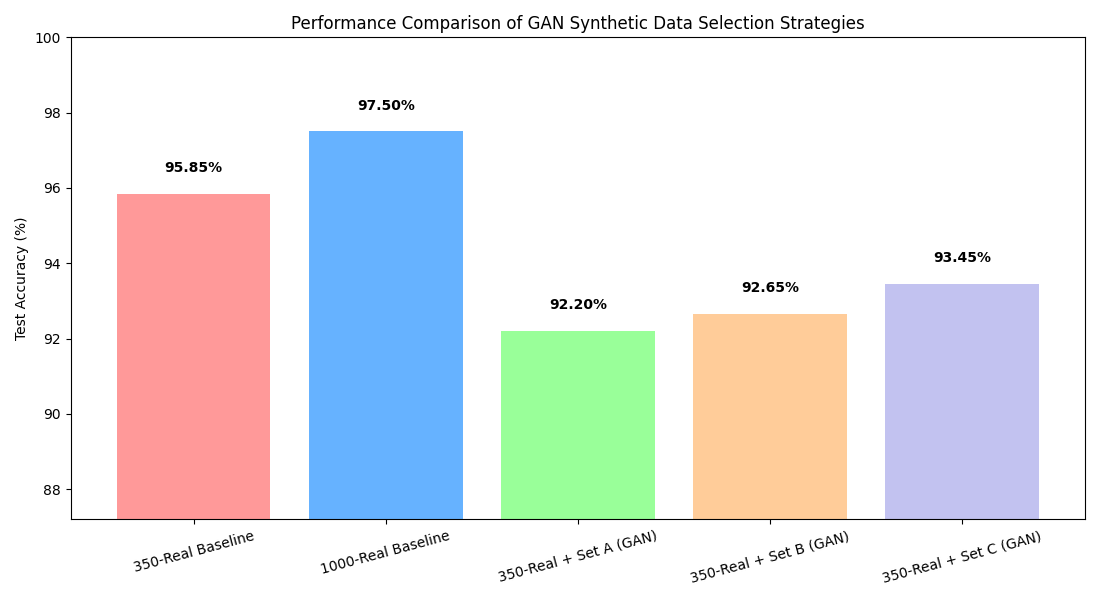
\includegraphics[width=0.85\textwidth]{../Problem_2_GAN/Outputs/6_Evaluation_Plots/gan_benchmarking_results.png}
    \caption{Performance comparison of GAN synthetic data selection strategies.}
    \label{fig:gan_benchmarking}
\end{figure}
